\documentclass[12pt]{article}

% Packages for styling and layout
\usepackage[table,xcdraw]{xcolor}
\usepackage{tikz}
\usepackage{geometry}
\geometry{margin=1in}

% Custom colors for your team
\definecolor{darkgrey}{RGB}{64,64,64}
\definecolor{maroon}{RGB}{128,0,0}

% Title styling
\newcommand{\teamtitle}{
    \centering
    \vspace{1em}
    
\begin{tikzpicture}
        \node[draw=none, fill=maroon, text width=\textwidth, minimum height=2cm, align=center] {
            \textcolor{white}{\Huge \bfseries FRC-1721 Bingo}\\[0.5em]
            \textcolor{white}{\large 2025}
        };
    \end{tikzpicture}
    \vspace{1em}
}

% Bingo grid dimensions
\newcommand{\bingosize}{5} % 5x5 grid

% Bingo cell styling
\newcommand{\bingocell}[1]{
    \node[draw, thick, minimum size=3cm, align=center] {#1};
}

\begin{document}

\teamtitle

\begin{center}
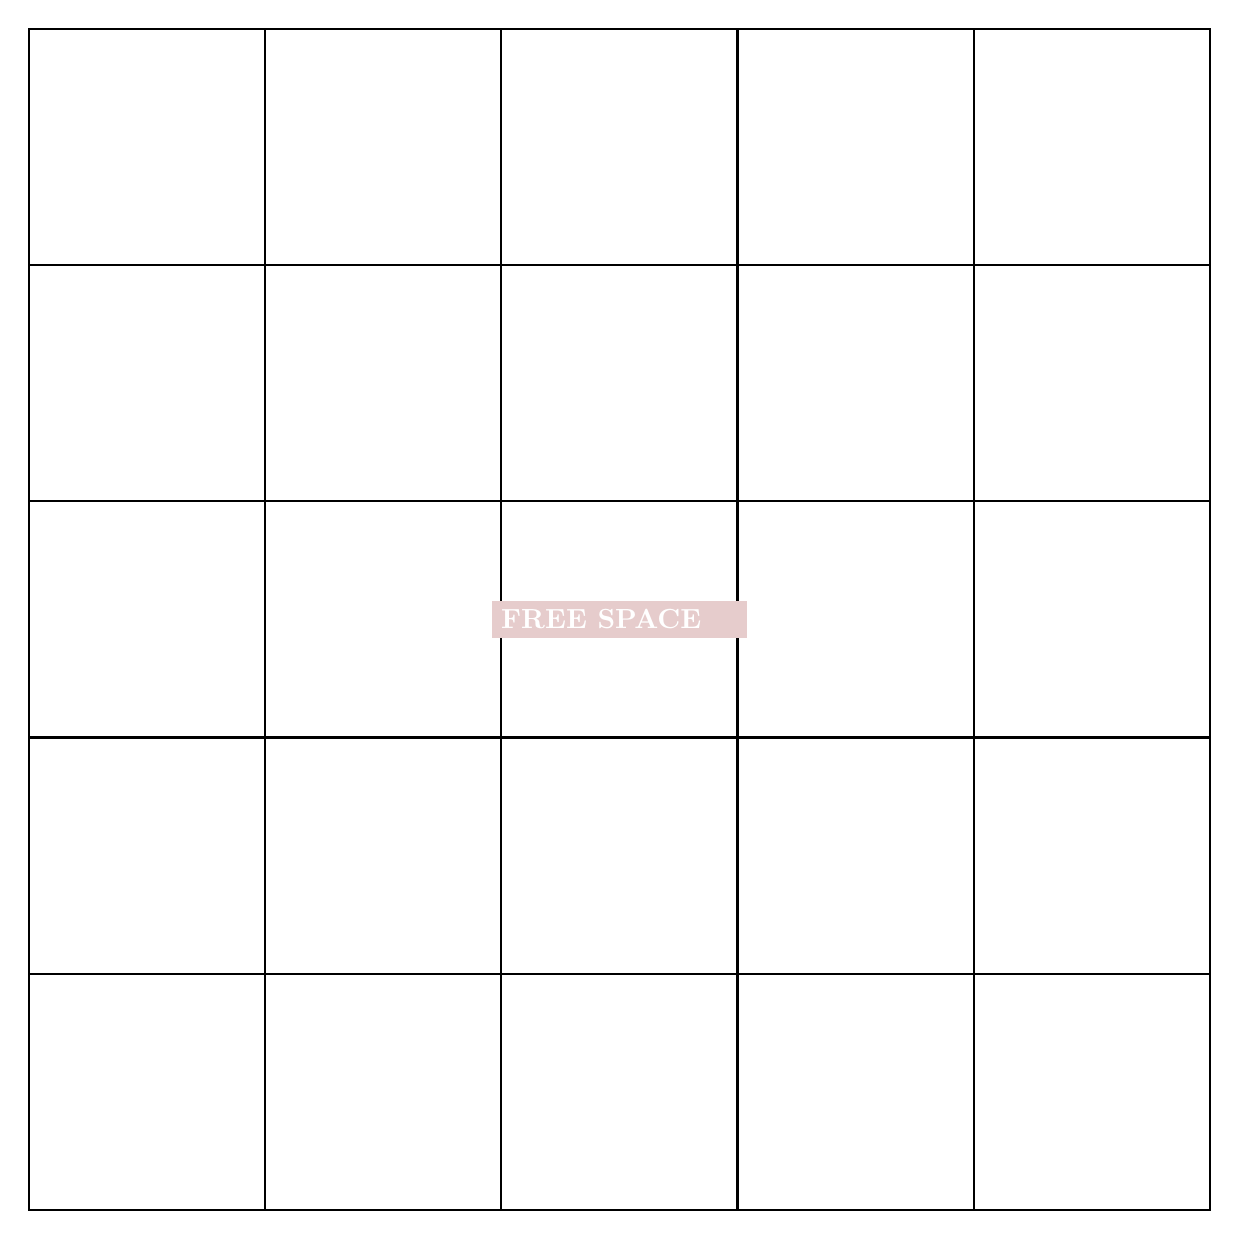
\begin{tikzpicture}[x=3cm, y=3cm]
    % Draw grid
    \foreach \x in {0,...,\numexpr\bingosize-1\relax} {
        \foreach \y in {0,...,\numexpr\bingosize-1\relax} {
            \node[draw, thick, minimum size=3cm, align=center] at (\x, -\y) {\phantom{X}};
        }
    }

    % Cells
    \node[fill=maroon!20, text=white, text width=3cm, font=\bfseries] at (2, -2) {FREE SPACE};
    % \node[thick, text width=3.5cm, align=center] at (1, -1) {Team Stands Around the Broken Robot};

    % {AUTOPOP ANCHOR}


\end{tikzpicture}
\end{center}

\end{document}
